% Regular polygons
\documentclass[tikz,border=10pt]{standalone}
\usepackage{tikz}
\usetikzlibrary{shapes,calc,arrows,through,intersections}
\usetikzlibrary{decorations.pathmorphing}
\usetikzlibrary{decorations.markings}
\usepackage{calc}

\begin{document}

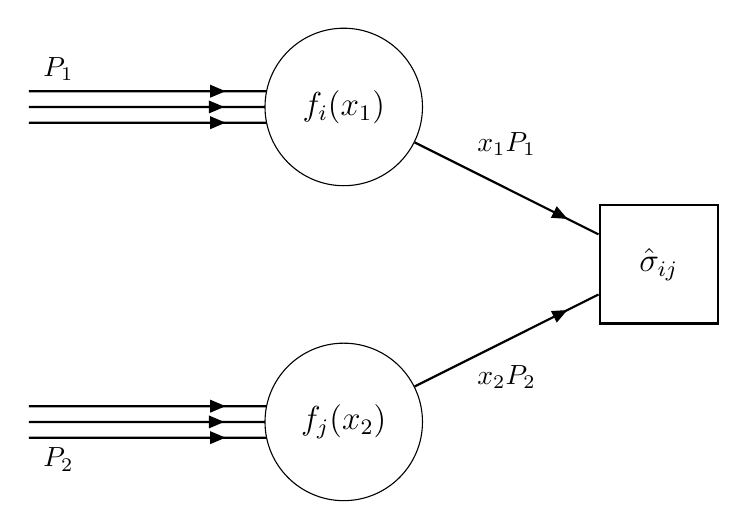
\begin{tikzpicture}
  % \draw[step=1.0,thin,gray!40] (0,0) grid (10,10);

  \node[circle, draw, minimum size=2cm] (circleANode) at  (4,8) {\large $f_i(x_1)$};
  \node[circle, draw, minimum size=2cm] (circleBNode) at  (4,4) {\large $f_j(x_2)$};
  \path[name path=circleA, thick] (4,8) circle [radius=1];
  \path[name path=circleB, thick] (4,4) circle [radius=1];

  \draw[thick] (8,6) node[draw,rectangle,minimum width=1.5cm,minimum height=1.5cm] (C) {\large $\hat \sigma_{ij}$};

  \path[name path=A1] (0,8.2) -- (4,8.2);
  \draw [postaction={decorate, decoration={markings, mark=at position 0.8 with {\arrow[scale=0.7,xshift=3.333pt]{triangle 45}}}},name intersections={of=A1 and circleA}, thick]  (0,8.2) -- (intersection-1) node[above,very near start] {$P_1$};
  \path[name path=A2] (0,8.0) -- (4,8.0);
  \draw [postaction={decorate, decoration={markings, mark=at position 0.8 with {\arrow[scale=0.7,xshift=3.333pt]{triangle 45}}}},name intersections={of=A2 and circleA}, thick]  (0,8.0) -- (intersection-1);
  \path[name path=A3] (0,7.8) -- (4,7.8);
  \draw [postaction={decorate, decoration={markings, mark=at position 0.8 with {\arrow[scale=0.7,xshift=3.333pt]{triangle 45}}}},name intersections={of=A3 and circleA}, thick]  (0,7.8) -- (intersection-1);

  \path[name path=B2] (0,4.2) -- (4,4.2);
  \draw [postaction={decorate, decoration={markings, mark=at position 0.8 with {\arrow[scale=0.7,xshift=3.333pt]{triangle 45}}}},name intersections={of=B2 and circleB}, thick]  (0,4.2) -- (intersection-1);
  \path[name path=B2] (0,4.0) -- (4,4.0);
  \draw [postaction={decorate, decoration={markings, mark=at position 0.8 with {\arrow[scale=0.7,xshift=3.333pt]{triangle 45}}}},name intersections={of=B2 and circleB}, thick]  (0,4.0) -- (intersection-1);
  \path[name path=B2] (0,3.8) -- (4,3.8);
  \draw [postaction={decorate, decoration={markings, mark=at position 0.8 with {\arrow[scale=0.7,xshift=3.333pt]{triangle 45}}}},name intersections={of=B2 and circleB}, thick]  (0,3.8) -- (intersection-1) node[below,very near start] {$P_2$};

  \draw [thick,postaction={decorate, decoration={markings, mark=at position 0.8 with {\arrow[scale=0.7,xshift=3.333pt]{triangle 45}}}}]  (circleANode) -- (C) node[midway,above,inner sep=.4cm] {$x_1P_1$};
  \draw [thick,postaction={decorate, decoration={markings, mark=at position 0.8 with {\arrow[scale=0.7,xshift=3.333pt]{triangle 45}}}}]  (circleBNode) -- (C) node[midway,below,inner sep=.3cm] {$x_2P_2$};
\end{tikzpicture}

\end{document}
